
% ~~~~~~~~~~~~~~~~~~~~~~~~~~~~~~~~~~~~~~~~~~~~~~~~~
\section{CALCUL DIFFÉRENTIEL}
% ~~~~~~~~~~~~~~~~~~~~~~~~~~~~~~~~~~~~~~~~~~~~~~~~~
\pagenumbering{arabic}
\setcounter{page}{1}
% =================================================
\subsection{Échauffement}
% =================================================

% -------------------------------------------------
\begin{exo}
    Déterminer le domaine de définition maximal des expressions suivantes :
    \begin{examplescol}{2}
        \item $f_1(x) = x^2 +x+1$
        \item $f_2(x) = \sqrt {x-1}$
        \item $f_3(x) = \sqrt{\frac{2 + 3 x}{5-2x}}$
        \item $f_4(x) = \ln (4 x + 3)$
    \end{examplescol}
\end{exo}

% -------------------------------------------------
\begin{exo}
    Soit $f : x\mapsto -x^2+x+2$.
    \begin{enumerate}
        \item Déterminer les racines de $f$.
        \item Dresser le tableau des variations de $f$ et donner ces intervalles de monotonie.
        \item Tracer le graphe de la fonction $f$. Donner son image.
        \item Résoudre les inégalités $f(x) \leq 0$, $f(x) > 1$, $f(x) < 5$.
    \end{enumerate}
\end{exo}

% -------------------------------------------------
\begin{exo}
    Soit $f : x\mapsto \sqrt{x+1}$.
    \begin{enumerate}
        \item Déterminer le domaine de définition de la fonction $f$.
        \item Dresser le tableau des variations de $f$ et donner ces intervalles de monotonie.
        \item Tracer le graphe de la fonction $f$.
        \item Résoudre les inégalités $f(x) \leq 1$, $f(x) > 2$.
    \end{enumerate}
\end{exo}

% -------------------------------------------------
\begin{exo}
    Résoudre les équations suivantes~:
    \begin{examplescol}{2}
        \item $3\ln \left( x+4\right) =9$
        \item $\ln \left( x^{2}\right) +3\ln \left( x\right) =5$
        \item $\ln \left( x+2\right) +\ln \left( x\right) =3$
        \item $\left[ \ln \left( x\right) \right] ^{2}-2=0$

        \item $e^{x}=e^{1-x}$
        \item $e^{3x}-2e^{-x}=0$
        \item $2^{x^{2}}=4\times2^{-x}$
        \item $3^{x}-2^{x^{2}}=0$
    \end{examplescol}
\end{exo}

% -------------------------------------------------
\begin{exo}
    Calculer les limites suivantes.
    \begin{examplescol}{3}
        \item $\displaystyle \underset{x \to +\infty}{\lim} \frac{e^{x}}{x}$
        \item $\displaystyle \underset{x \to 1}{\lim} \frac{x-1}{\ln(x)} $
        \item $\displaystyle \underset{x \to +\infty}{\lim} \frac{x^{2}+3}{2x^{2}+x+1} $
        \item $\displaystyle \underset{x \to 0}{\lim} \frac{\sin(x)}{x} $
        \item $\displaystyle \underset{x \to 1}{\lim} \frac{x-1}{x+1} $
        \item $\displaystyle \underset{x \to +\infty}{\lim} x^{\frac{1}{x}} $
        \item $\displaystyle \underset{x \to +\infty}{\lim} x-\ln(x) $
        \item $\displaystyle \underset{x \to +\infty}{\lim} x\tan(\frac{1}{x}) $
        \item $\displaystyle \underset{x \to +\infty}{\lim} \sqrt{x^{2}-x}-x $
    \end{examplescol}
\end{exo}

% -------------------------------------------------
\begin{exo}
    Étudier les fonctions suivantes.
    \begin{examplescol}{4}
        \item $\displaystyle \frac{x^{2}-x-2}{x-3} $
        \item $\displaystyle x+e^{-x} $
        \item $\displaystyle \sqrt{\frac{x+1}{x+2}} $
        \item $\displaystyle x^{2}-8\ln(x)+1 $
        \item $\displaystyle \ln(x-\frac{1}{x}) $
        \item $\displaystyle x^{\frac{1}{x}} $
        \item $\displaystyle \frac{2x^{3}}{x^{2}-1} $
        \item $\displaystyle \ln(x+1)-\ln(x)+x $
    \end{examplescol}
\end{exo}


% =================================================
\subsection{Problèmes d'optimisation}
% =================================================

% -------------------------------------------------
\begin{exo}

    \image{r}{7cm}{-14mm}{-14mm}{drawings/poisson.tikz}

    L'énergie dépensée par un poisson pour remonter une distance $d$ d'un courant de vitesse $u$ à la vitesse $v$ est donnée par
    $$
        E(v) = v^{3}\frac{d}{v-u}.
    $$

    \begin{enumerate}
        \item Quel est le domaine de définition de cette fonction ?

        \item On se restreindra ici au domaine $]u,+\infty[$. Expliquer pourquoi.

        \item Étudier la fonction $E$ sur $]u,+\infty[$.

        \item En déduire la vitesse $v$ qui minimise l'énergie $E(v)$, puis calculer cette énergie minimale.
    \end{enumerate}
\end{exo}

% -------------------------------------------------
\begin{exo}

    \image{r}{5cm}{-11mm}{-21mm}{drawings/decoupe_boite.tikz}

    On souhaite construire un casier rectangulaire en découpant quatre carrés de même taille aux coins d'une feuille cartonnée et en rabattant les bords restants. La feuille mesure $42$ cm de long et $32$ cm de large. Le volume du casier dépendra de la taille des carrés découpés. Dans cet exercice on cherche à trouver la taille des carrés qui maximisera le volume du casier.

    \begin{enumerate}
        \item On note $x$ la longueur d'un des côtés des carrés. Montrer que l'on a $0 < x < 16$.

        \item Montrer que le volume $V$ s'exprime en fonction de $x$ sous la forme
        $$ V(x) = 4(336x - 37x^2 + x^3) $$

        \item Étudier la fonction $V$ sur $]0,16[$. En déduire la taille des carrés qui maximisera le volume du casier.

        \item Calculer le volume maximale du casier réalisable avec cette feuille.
    \end{enumerate}
\end{exo}

% -------------------------------------------------
\begin{exo}
    Un camion doit faire un trajet de 140 km. On sait que sa consommation en gazole est de $(4 + \frac{v^2}{1225})$ litres par heure, où $v$ désigne la vitesse du camion en km/h. Le prix du gazole est de 1 euro et 40 centimes par litre (en Belgique). Dans cet exercice, on cherche la vitesse du camion (supposée constante en fonction du temps) qui minimisera le prix de revient de la course.
    \begin{enumerate}
        \item Expliquer pourquoi le nombre de litres $N(v)$ consommés par le camion en 140 km, en fonction de $v$, est
            $$
                N(v) = (4 + \frac{v^2}{1225}) \frac{140}{v}.
            $$
        \item En déduire l'expression du prix de revient $P(v)$ (en euros) de la course en fonction de $v$.
        \item Étudier la fonction $P$ sur $]0,+\infty[$. En déduire la vitesse $v$ qui minimise le prix de revient de la course. Quelle est ce prix minimal ?
    \end{enumerate}
\end{exo}

% -------------------------------------------------
%\begin{exo}
%    Un campeur décide de se construire un tipi, c'est-à-dire une tente conique. Pour cela, il dispose de $S=9\pi$ mètres carrés de toile, soit environ 28m$^2$. Il veut que le volume habitable sous le tipi soit le plus grand possible.

%    \image{r}{4cm}{0mm}{-21mm}{drawings/tipi.tikz}
%    Si le tipi a un rayon au sol $x$ et une hauteur $h$, le volume habitable est donné par la formule
%    $$
%        V=\frac{1}{3}\pi x^2h
%    $$
%    et la superficie de toile utilisée vaut $\pi x\sqrt{x^2+h^2}=9\pi$.

%    \begin{enumerate}
%        \item  Montrer que $h=\sqrt{\frac{81}{x^2}-x^2}$.
%        \item En déduire que le volume habitable vaut
%        $$
%            V(x)=\frac{\pi x}{3}\sqrt{81-x^4}.
%        $$
%        \item Étudier la fonction $V$ en fonction de $x$ sur l'intervalle $[0,3]$.
%        \item Quel doit être le rayon au sol du tipi pour que le volume habitable soit maximal~? Quelle sera alors sa hauteur~?
%    \end{enumerate}
%\end{exo}

% -------------------------------------------------
\begin{exo}
Dans une ruche, chaque alv\'eole a une forme de prisme hexagonal dont la surface est donn\'ee, pour une longueur de c\^ot\'e
\(s\) et une hauteur \(h\) par 
\[A(\theta) = 6sh - \frac{3}{2}s^{2}\frac{\cos(\theta)}{\sin(\theta)}+\frac{3\sqrt{3}}{2}s^{2}\frac{1}{\sin(\theta)}\]
o\`u \(\theta\) d\'esigne l'angle au sommet du prisme.
\begin{center}
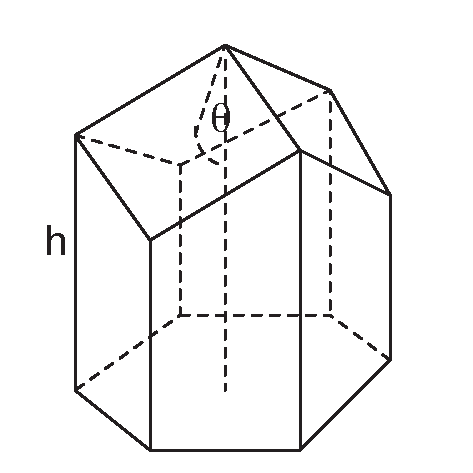
\includegraphics[width=6cm]{drawings/abeille.pdf}
\end{center}
\begin{enumerate}
\item Quelle est le domaine de d\'efinition de cette fonction ? 
\item On se restreindra ici au domaine $]0,\pi[$. Expliquer pourquoi. 
\item  Etudier la fonction $A$ sur $]0,\pi[$. 
\item En d\'eduire l'angle \(\theta\) qui minimise la surface $A(\theta)$ d'une telle alv\'eole et d\'eterminez, en fonction de \(s\) et \(h\), la surface correspondante.
\end{enumerate}

\textit{Dans la réalité, les alvéoles ont l'angle $\theta$ optimal à $\pm 2$ degrés près.}
\end{exo}


% =================================================
\subsection{Équations différentielles}
% =================================================

% -------------------------------------------------
\begin{exo}
    La variole est une maladie très contagieuse. Lorsqu'un individu est infecté, soit il meurt, soit il est immunisé pour le reste de sa vie. On a donc cherché à savoir s'il fallait inoculer la variole de façon préventive (et inoffensive) à toute la population.

    Si la variole a été inoculée, le nombre $P(x)$ d'individus encore vivants à l'âge $x$ (en décennies) satisfait l'équation différentielle suivante.

    \begin{eqnarray}\label{eqP}
        y'(x)=-\frac{x+1}{x+2}\,y(x)\quad\mathrm{pour}\quad x\ge 0.
    \end{eqnarray}

    \begin{enumerate}
        \item Soit $K>0$. Vérifier que la fonction définie par $P(x)=K(x+2)e^{-x}$ est solution de l'équation différentielle (\ref{eqP}).
        \item Montrer que $P(x)>0$ pour tout $x\ge 0$.
    \end{enumerate}

    \noindent Si la variole n'avait pas été inoculée, on aurait eu
    $$
        T(x)=\frac{K}{8}(7e^{x/8}+1)(x+2)e^{-\frac{9x}{8}} \qquad \text{individus d'âge } x.
    $$
    On pose $f(x)=\frac{T(x)}{P(x)}$ pour tout $x\ge 0$.

    \begin{enumerate}
        \item Montrer que $f(x)=\frac{1}{8}(7+e^{-x/8})$.
        \item Établir le tableau de variations de la fonction $f$ sur l'intervalle $[0,+\infty[$.
        \item A-t-on intérêt à inoculer préventivement la variole aux nourrissons?
    \end{enumerate}

    \textit{La variole a été éradiquée en 1979.}
\end{exo}

% -------------------------------------------------
\begin{exo}
    On observe une population de microbes se développant de manière malthusienne, c'est à dire dont le taux de croissance au temps $t$ (en heures) est proportionnel à la taille de la population $N(t)$.
    \begin{enumerate}
        \item
        En notant $k$ la constante de proportionnalité, donner une équation différentielle modélisant cette situation.
        \item
        Montrer que les fonctions $N(t) = Ce^{kt}$ (où $C$ est une constante) sont solutions de cette équation différentielle.
        \item
        Que représente $C$ ?
        \item
        Si $k= \ln 2$, que peut-on dire de la population au bout d'une heure ?
        \item
        Si $k = \ln 2$ et $N(0)=100$, quelle sera, d'après le modèle, la taille de la population au bout de 4 heures et 20 minutes ?
        \item
        Si $k = \ln 2$ et $N(0)=100$, au bout de combien de temps la population atteindra-t-elle 1000 individus ?
    \end{enumerate}
\end{exo}

% -------------------------------------------------
\begin{exo}
    On modélise le refroidissement d'une roche lors d'une éruption volcanique, en partant du principe que le taux de refroidissement est proportionnel à la différence de température entre la roche et l'air ambiant.
    On note $T_{a}$ la température de l'air ambiant et $T(t)$ la température (en degrés Celsius) de la roche au temps $t$ (en heures).
    \begin{enumerate}
        \item
        En notant $k>0$ la constante de proportionnalité, donner une équation différentielle modélisant cette situation.
        \item
        Montrer que les fonctions $T(t) = C\,e^{-kt}+T_{a}$ (où $C$ est une constante) sont les solutions de cette équation différentielle.
        \item
        Que représente $C$ ?
        \item
        Si $k=\ln 3$, $T_{a} = 50$ et $T(0) = 500$, quelle sera, d'après le modèle, la température de la roche après 30 minutes ?
        \item
        Si $k=\ln 3$, $T_{a} = 50$ et $T(0) = 500$, au bout de combien de temps la température de la roche sera-t-elle de 100 degrés Celsius ?
    \end{enumerate}
\end{exo}

% -------------------------------------------------
\begin{exo}
    On considère une population de bactéries. On note $x(t)$ le nombre de bactéries à l'instant $t$, et $x_0$ le nombre de bactéries au début de l'expérience (instant $t=0$).

    Lorsque la bactérie est isolée, l'effectif $x(t)$ possède une vitesse de
    croissance $x'(t)$ proportionnelle à $x(t)$ (on note $\alpha>0$ ce coefficient de proportionnalité). Lorsqu'une certaine toxine est présente dans le milieu de culture en quantité $y(t)$, le coefficient de proportionnalité $\alpha$ est diminué de la quantité $y(t)$.
    On suppose que $y(t)$ croit de façon affine en fonction du temps, par exemple $y(t) = 2t + 1$.
    \begin{enumerate}
        \item Expliquer pourquoi $x(t)$ est solution du problème
        \begin{eqnarray}
            x'(t) & = & (\alpha - 2t -1)x(t) \label{ncdiffx} \\
            x(0)  & = & x_0 \label{cix}
        \end{eqnarray}
        Dans la suite, on suppose qu'il y a des bactéries lorsqu'on débute l'expérience: $x_0>0$.
        \item On cherche une solution sous la forme $x(t) = e^{p(t)}$ où $p(t)=at^2+bt+c$ est un polynôme de degré 2. A quelle condition sur les coefficients de $p$ l'équation (\ref{cix}) est-elle vérifiée? A quelle condition sur les coefficients de $p$ l'équation (\ref{ncdiffx}) est-elle vérifiée? En déduire $x(t)$.
        \item On suppose $\alpha > 1$. Étudier les variations de la fonction $x(t)$. A quel moment la population de bactéries est-elle maximale ?
        La population a-t-elle une chance de survie en grand temps ?
    \end{enumerate}
\end{exo}

% -------------------------------------------------
\begin{exo}
    \noindent On considère le problème
    \begin{eqnarray}
        y'(t)&=&-t^2y(t)\quad\mathrm{pour}\ t\ge 0 \label{eq}\\
        y(0)&=&y_0\label{ci}
    \end{eqnarray}
    \begin{enumerate}
        \item Montrer que la fonction constante $y(t)=0$ est solution de (\ref{eq}). Y a-t-il d'autres solutions constantes?
        \item On suppose que $y$ est une solution de (\ref{eq}) et (\ref{ci}), et on
        suppose $y_0>0$.
        \begin{enumerate}
            \item  Montrer que $y(t)>0$ pour tout $t\ge 0$ ({\it on admettra que les graphes
            de deux solutions distinctes de (\ref{eq}) ne se coupent jamais}).
            \item Montrer que $y$ est décroissante sur $[0;+\infty[$. En déduire que $y(t)$ a une limite quand $t\to +\infty$.
        \end{enumerate}
        \item On pose $u(t)=at^3+b$ et $Y(t)=e^{u(t)}$, où $a$ et $b$ sont des constantes.
        \begin{enumerate}
            \item Calculer $u'(t)$ et $Y'(t)$.
            \item Déterminer la constante $a$ pour que $Y(t)$ soit solution de (\ref{eq}).
            \item Calculer $Y(0)$. Comment faut-il choisir $b$ pour avoir $Y(0)=y_0$?
            \item Calculer $\lim_{t\to +\infty}Y(t)$, en prenant pour $a$ et $b$ les valeurs trouvées dans les questions précédentes.
        \end{enumerate}
    \end{enumerate}
\end{exo}

% -------------------------------------------------
\begin{exo}
    On étudie la progression d'une maladie contagieuse dans une population donnée. On note $x(t)$ la
    proportion des personnes malades à l'instant $t$, $y(t)$ celle des personnes saines, et $y_0$ la proportion de personnes saines à l'instant initial $t=0$. On a donc
    $x(t) + y(t) = 1$ pour tout $t \geq 0$.

    On suppose que la vitesse de propagation de la maladie $x'(t)$ est proportionnelle
    au produit $x(t)y(t)$ (ce qui signifie que la maladie se propage par contact).
    \begin{enumerate}
        \item Expliquer pourquoi il existe une constante $K>0$ telle que $y(t)$ soit solution du problème
        \begin{eqnarray}
            y'(t) &=& -K y(t)(1-y(t)) \label{diffy}\\
            y(0)  &=& y_0\label{ciy}
        \end{eqnarray}
        pour tout $t \geq 0$.
        \item Chercher les solutions constantes de l'équation (\ref{diffy}).\\

        \noindent Dans la suite, on supposera $0 < y_0 < 1$.
        \item Déduire de l'équation différentielle (\ref{diffy}) que la fonction $y$ est décroissante ({\it indication: étudier le signe de $y'(t)$ en admettant que les graphes de
        deux solutions distinctes de (\ref{diffy}) ne se coupent jamais}).
        \item En déduire que $\lim_{t \rightarrow +\infty} y(t) = l$ avec $l \in \mathbb{R}$. On admet que dans ce cas
        $ y'(t)\xrightarrow[t\to +\infty]{}0$. En déduire, en utilisant (\ref{diffy}), que $l=0$.
        La population peut-elle survivre sans intervention extérieure ?
        \item On considère la fonction
        \begin{equation}
            Y(t) = \frac{1}{ 1 + C\,e^{Kt} } \label{y}.
        \end{equation}
        \begin{enumerate}[(i)]
            \item Montrer que lorsque $C \ge 0$, $Y(t)$ est défini pour tout $t \geq 0$.
            \item Montrer que $Y(t)$ est solution de l'équation (\ref{diffy}). 
            \item Trouver $C$ pour que $Y(t)$ satisfasse aussi (\ref{ciy}). %\frac{1-y_0}{y_0}
            \item Répondre à la question (d) en utilisant l'expression (\ref{y}).
        \end{enumerate}
    \end{enumerate}
\end{exo}

% -------------------------------------------------
\begin{exo}
    On étudie l'évolution d'une population de thons en Alaska. On note $p(t)$ le nombre (en centaines) de thons à l'instant $t\ge 0$ (en heures). On observe que cette population a un taux de croissance de 3\% à chaque instant $t$. Cette population subit les assauts d'une pêche intensive qui réduit la population de $10^{-2}p(t)^2$ thons par heure. De plus, à chaque heure, 2 thons quittent la population pour des causes naturelles. On obtient alors l'équation différentielle satisfaire par $p(t)$:
    \begin{equation}\label{eqthons}
        p'(t)=10^{-2}(-p(t)^2+3p(t)-2)
    \end{equation}
    \begin{enumerate}
        \item Expliquer chaque terme de l'équation (\ref{eqthons}) à l'aide du texte introductif.
        \item Calculer les solutions de l'équation $-p^2+3p-2=0$.
        \item En déduire les solutions constantes de l'équation (\ref{eqthons}).
        \item On considère maintenant la solution $p(t)$ de (\ref{eqthons}) vérifiant $p(0)=10$.
        \begin{enumerate}[(i)]
            \item Montrer que  le nombre de thons diminue au cours du temps en admettant que les graphes de
            deux solutions distinctes de (\ref{eqthons}) ne se coupent jamais.
            \item Montrer que $\displaystyle \lim_{t\to +\infty}p(t)=l$ avec $l \in \mathbb{R}$, puis calculer $l$ en admettant que $\displaystyle \lim_{t\to +\infty}p'(t)=0$. La population de thons a-t-elle une chance de survie en grand temps?
        \end{enumerate}
    \end{enumerate}
\end{exo}

% -------------------------------------------------
\begin{exo}
     On considère le problème représenté par les deux équations suivantes:
            \begin{eqnarray}
                y'(t)&=&(y(t)-1)^2(y(t)+1)\label{eqpoly}\\
                y(0)&=&0 \label{cipoly}
            \end{eqnarray}
            et l'on suppose qu'il existe une fonction $y:\R^+\to\R$ solution de ce problème.
            \begin{enumerate}
                \item Chercher les solutions constantes de l'équation différentielle (\ref{eqpoly}).
                \item Montrer que la solution $y$ du problème est croissante sur $\R^+$ ({\it indication: étudier le signe de $y'(t)$ en admettant que les graphes de
                deux solutions distinctes de (\ref{eqpoly}) ne se coupent jamais}).
                \item En déduire que $\displaystyle \lim_{t\to +\infty}y(t)=l$ avec $l \in \mathbb{R}$. Calculer $l$ en admettant que $\displaystyle \lim_{t\to +\infty}y'(t)=0$.
            \end{enumerate}
  
\end{exo}

% -------------------------------------------------
\begin{exo}
    Lorsqu'une nouvelle espèce s'introduit dans un écosystème, elle évolue d'abord lentement. Son rythme de croissance s'accélère ensuite à mesure qu'elle s'adapte, puis ralentit quand le nombre d'individus $u$ devient trop important compte tenu des ressources disponibles.
    Pour ce type d'évolution, on utilise le modèle de Gompertz suivant~:
    \begin{eqnarray}
        & & u'(t)= -u(t)\ln(u(t)) \label{Gomp}\\
        & & u(0)=u_0 \label{ciu}
    \end{eqnarray}
    où $u_0$ désigne le nombre d'individus introduits au départ dans l'écosystème.
    \begin{enumerate}
        \item
        Chercher les solutions constantes de l'équation (\ref{Gomp}).
        \item Déduire de l'équation différentielle (\ref{Gomp}) que la fonction $u$ est décroissante si $u_0>1$, et croissante si $0<u_0<1$ ({\it indication: étudier le signe de $u'(t)$ en admettant que les graphes de
        deux solutions distinctes de (\ref{Gomp}) ne se coupent jamais}).
        \item
        En déduire que $l = \underset{t \to +\infty}\lim u(t)$ existe.
        \item
        Que vaut $l$ ? La population va-t-elle survivre ?
        \item On considère la fonction $U(t)=e^{Ce^{-t}}$ (où $C$ est une constante).
        \begin{enumerate}[(i)]
            \item Montrer que $U$ est solution de (\ref{Gomp}) et que $U(0)>0$.
            \item Trouver $C$ pour que la fonction $U$ soit solution du problème (\ref{Gomp}-\ref{ciu}). 
            \item Répondre à la question (d) en utilisant l'expression de $U(t)$.
        \end{enumerate}
    \end{enumerate}
\end{exo}


% ~~~~~~~~~~~~~~~~~~~~~~~~~~~~~~~~~~~~~~~~~~~~~~~~~
\finchapitre
